%!TEX root = ../document.tex

\section{Final Prototype}
\label{sec:FINAL_PROTOTYPE}
Our final prototype, we came up with after the user testing, is a mock-up for an Eclipse plug-in targeting aiming at the observed needs of database developers. The reader can get an impression on how it could look like in Figure \ref{fig:final_prototype_overview}.
\begin{figure}
\begin{centering}
    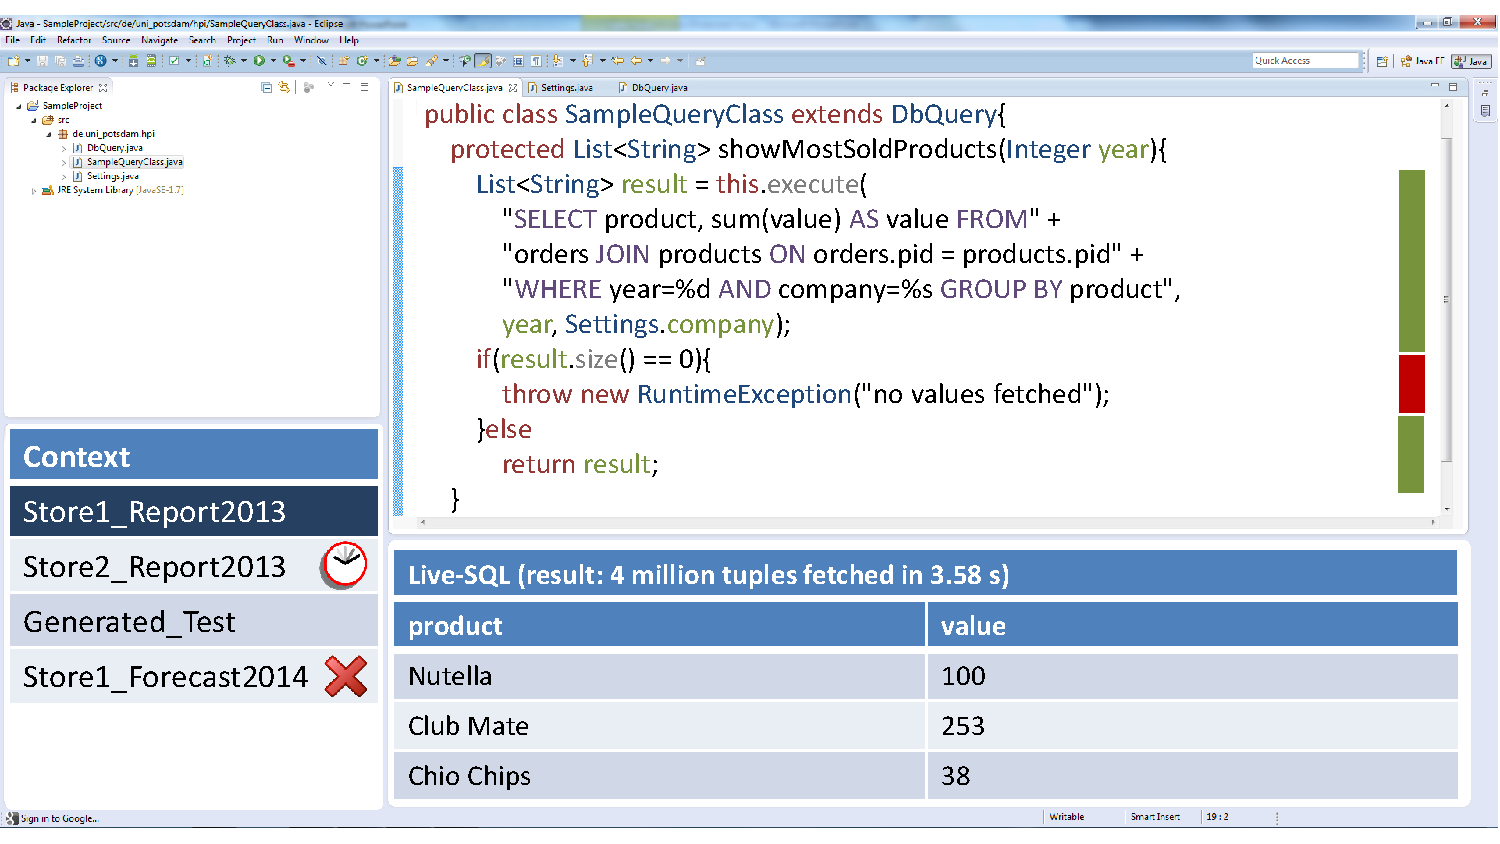
\includegraphics[width=1.0\linewidth]{images/final_prototype}
    \caption{Overview of the final prototype}
    % #selfrespect
    \label{fig:final_prototype_overview}
\end{centering}
\end{figure}
The plug-in consists mainly of 3 parts visible in the ui:
\begin{description}
	\item [Code-Editor] The code editor is mainly the standard Eclipse built-in editor, but with some enhancements like syntax-highlighting for in-line SQL and a instant code-coverage indication on the right side of the editor's pane. This indicates the branches of the code that will be executed depending on the current selected context.
	\item [Live-SQL] In the Live-SQL frame on the bottom of the IDE the developer has instant data access on the underlying database tables and views. It is also possible to explore the result sets of sub-queries. Furthermore the data is fortified with runtime information and data heuristics as you can see later.
	\item [Context-Browser] In the Context-Browser can switch instantly between different contexts and also gets indications on interesting and important contexts, like those evoking failures or runtime slow-downs.
\end{description}
In the following section we want to show the main features of the customized IDE and how the user can easily interact with this new environment.\\
As a main goal we wanted to make data context all time available to the developer, so the instant access on the underlying database is easy every time in the development process and doesn't need any break out of the ''flow'' as it would be nowadays. Therefore the user just selects any table, view or sub-select in his SQL-statement and gets an preview of the data immediately as you can see in Figure \ref{fig:final_prototype_instant}. Furthermore the system could provide meaningful visualizations of the data and give hints on performance issues, like the size and the fetch time of the relation.
\begin{figure}
\begin{centering}
    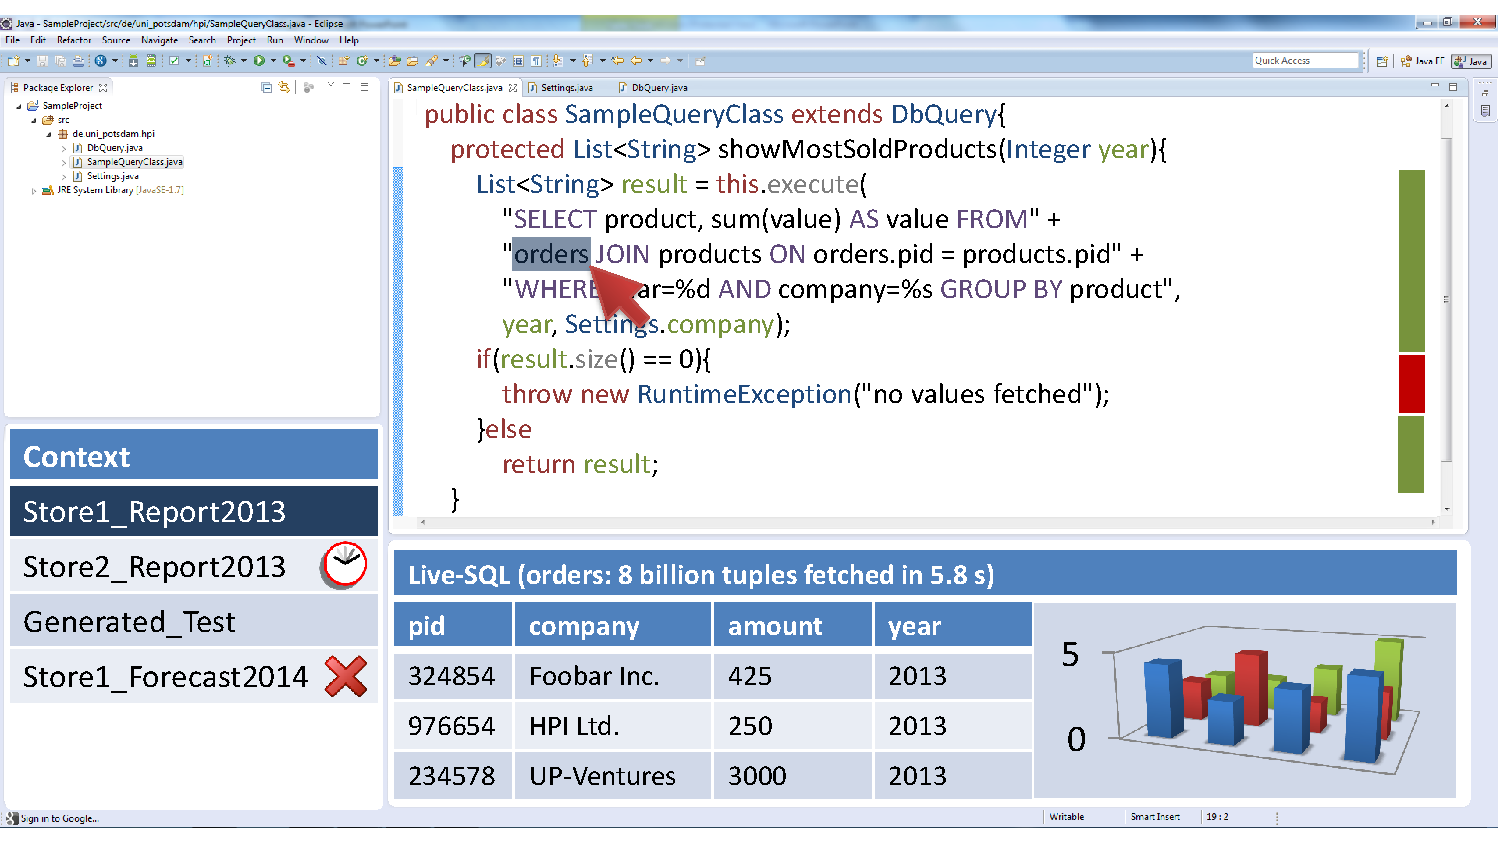
\includegraphics[width=1.0\linewidth]{images/instant}
    \caption{Instant data inspection of relations and sub-queries}
    % #selfrespect
    \label{fig:final_prototype_instant}
\end{centering}
\end{figure}
In the Context Browser the user gets indications for salient contexts, like the Context ``Store2\_Report2013'' in the given example. The little alarm clock behind it shall indicate that the developer should check this certain context because it was analyzed to be comparatively slow during runtime. The developer can now easily select this one in the browser and gets immediate feedback in the Live-SQL pane in the bottom, where he can see that the fetch time for the result relation is relatively slow. As a response he now could adapt the SQL-statement towards the  output intended by the overlying method (see the red red highlighted code in Figure \ref{fig:final_prototype_slow}). While the doveloper changes the code in the editor pane, the Live-SQL viewer displays a diff between the resulting relation before and after the code change. Due to the decreasing fetch time of the newly described query the performance indicator in the Context Browser would disappear and this issue is solved.\\
\begin{figure}
\begin{centering}
    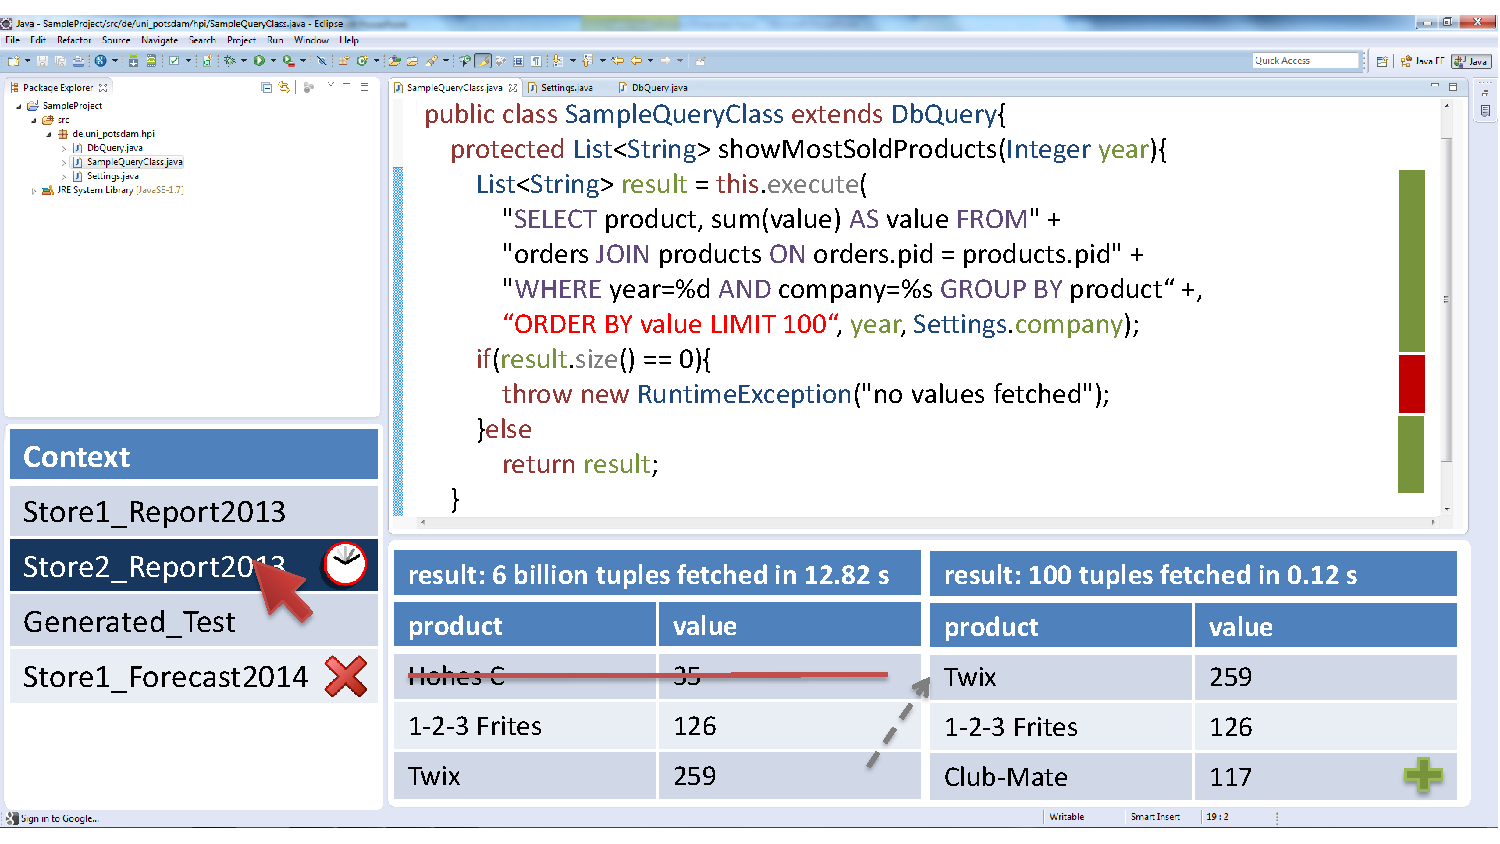
\includegraphics[width=1.0\linewidth]{images/slow}
    \caption{Performance flaw indication}
    % #selfrespect
    \label{fig:final_prototype_slow}
\end{centering}
\end{figure}
Because of the fact that a context in our supposed system is not only a database state but also runtime information of the code, we are also able to warn the developer about failure states his software would reach for special input combinations. Such an exceptional runtime context is displayed in Figure \ref{fig:final_prototype_error}, namely ``Store1\_Forecast2014''. Here the result set is empty, which directly has impact on the surrounding code of the query. This is indicated to the user by marking the covered branches differently than in the previous examples. Because of the 0 fetched rows from the database a runtime error is thrown in the methods, which is the failure state indicated by the red cross in the Context Browser for this example. The variable that is causing this faulty branch execution is the method's parameter ``year'' which is indicated to the developer by highlighting it red. While hovering over this variable he can get the value of it to better understand the failure. Now he has different possibilities for things he can do next. He could adapt the value of the input variable to better understand the error or he could easily mock the result data just by inserting tuples in the Live-SQL tab and therefore fore another branch execution.\\
\begin{figure}
\begin{centering}
    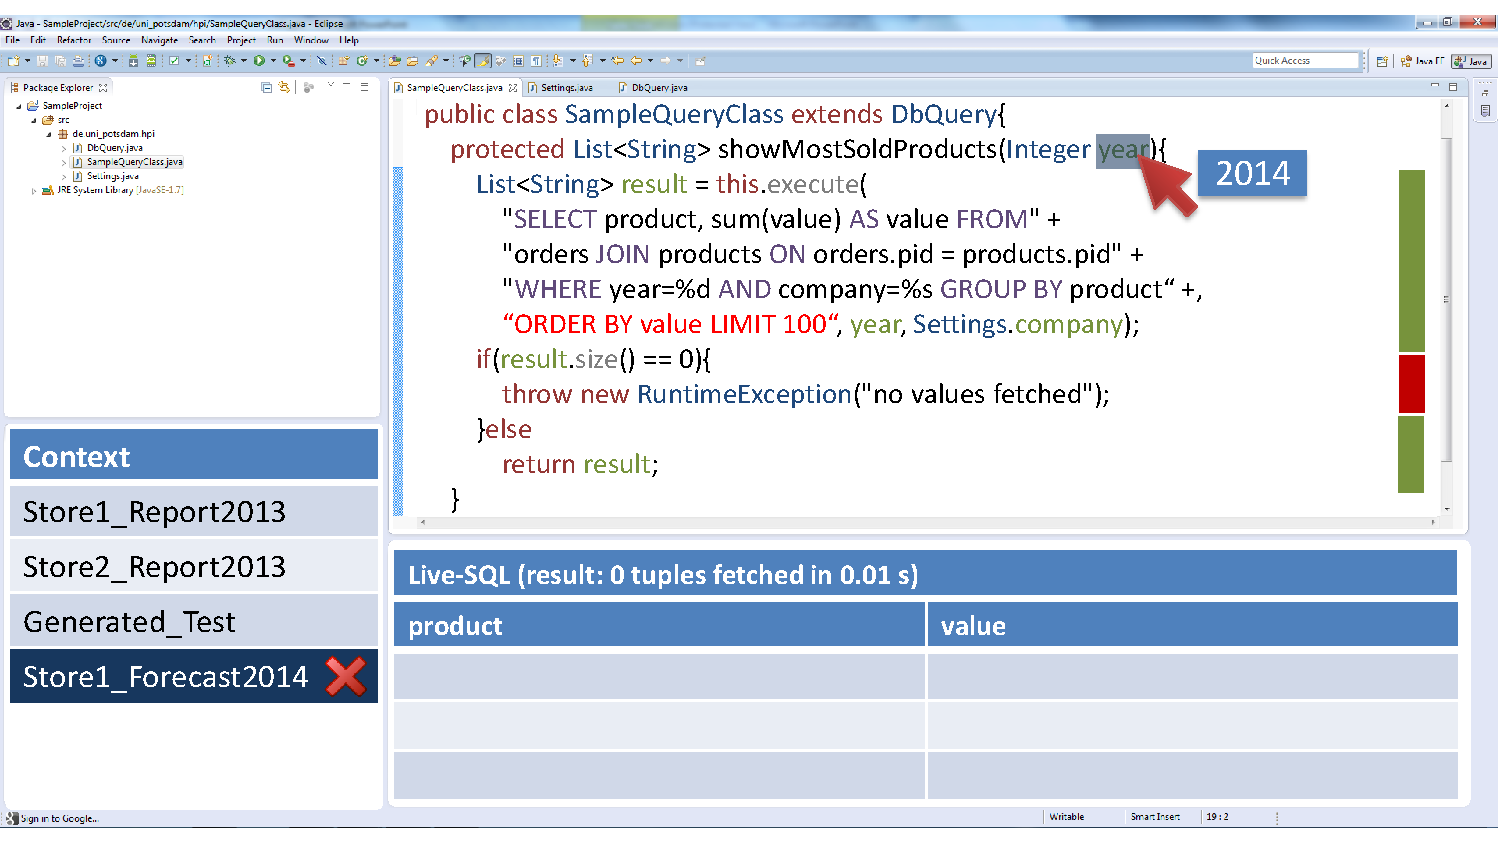
\includegraphics[width=1.0\linewidth]{images/error}
    \caption{Runtime-error indication and code coverage}
    % #selfrespect
    \label{fig:final_prototype_error}
\end{centering}
\end{figure}